\documentclass{article}
\usepackage{float}
\usepackage[margin = 2cm]{geometry}
\usepackage{graphicx}
\usepackage{bm}
\usepackage{amsmath,amssymb,amsfonts,amsthm}
\setlength{\parindent}{0pt}

\newcommand{\spacer}[1][8pt]{
    \par\vspace{#1}
}

\author
{
    Mattia Boscolo Meneguolo - 2066700, \\
    Matteo Cuzzolin - 2066701
}
\title{Tesina di Fondamenti di Controlli Automatici, A.A. 2024}
\date{}
\begin{document}
\maketitle

\begin{figure}[!htbp]
    \centering
    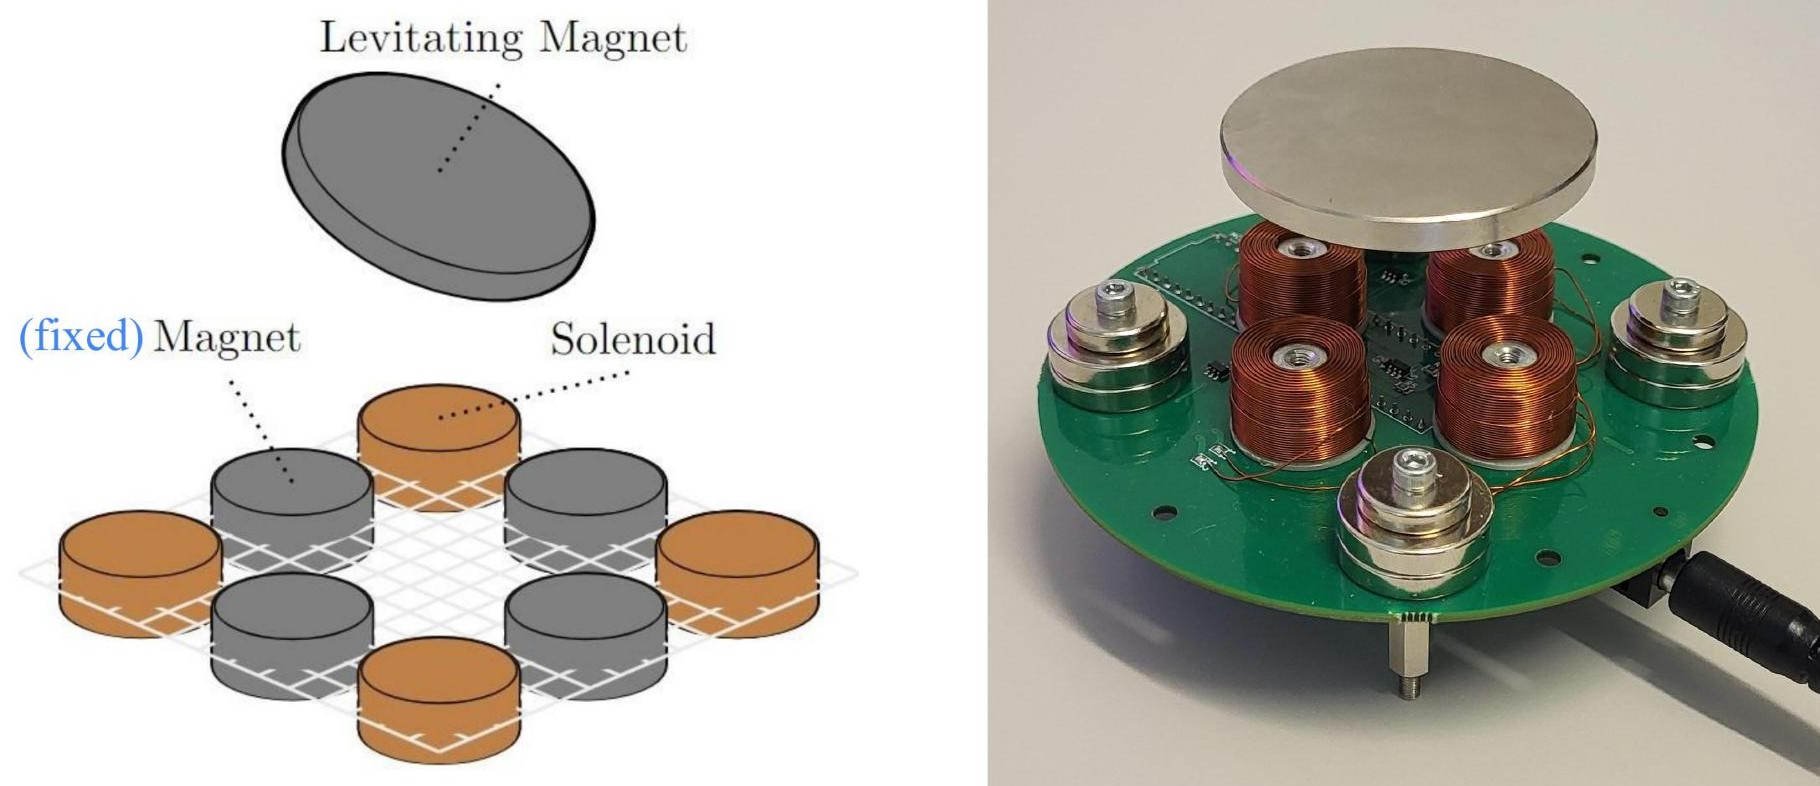
\includegraphics[width = 0.8\textwidth]{Images/maglev-system-schematics}
    \caption{Rappresentazione del sistema - Implementazione del sistema}
    \label{fig:rappresentazione_sistema}
\end{figure}

Sia $\tilde{z}(t) = z(t) - \overline{z}$ dove $z(t)$ è la posizione del magnete e $\overline{z}$ è la posizione del magnete all'equilibrio.

La trasformata di laplace di $\tilde{z}$ è:
$$\tilde{Z}(s) = \frac{b_s}{\overline{z}ms^2+\overline{z}ds+mg}I(s)+\frac{(ms+d)\tilde{z}(0)+m\tilde{z}'(0)}{ms^2+ds+\frac{mg}{\overline{z}}}$$

\section{Esercizio 1}
Studiamo la risposta libera, infatti in questo caso $i(t) = 0 \:\forall t$. Ipotizziamo anche che $\tilde{z}'(0) = 0$

$\tilde{Z}(s) =\frac{(ms+d)\tilde{z}(0)}{ms^2+ds+\frac{mg}{\overline{z}}}$

\spacer
Secondo la regola di Cartesio il polinomio al denominatore è stabile infatti tutti i coefficienti sono non nulli e positivi.

\spacer
Tuttavia dalle prime elaborazioni su mathlab risulta evidente che il sistema impiega un lungo periodo di tempo per assestarsi alla posizione di equilibrio.
Dato che vogliamo svolgere diverse simulazioni per mostrare che il sistema raggiunge l'equilibrio al variare di $\tilde{z}(0)$ aumenteremo il valore di d a 0.1 così da rendere più veloci le simulazioni.

\spacer
Questo è un esempio di una simulazione con $\tilde{z}(0)=0.35$ e $d=0.1$

\begin{figure}[H]
    \centering
    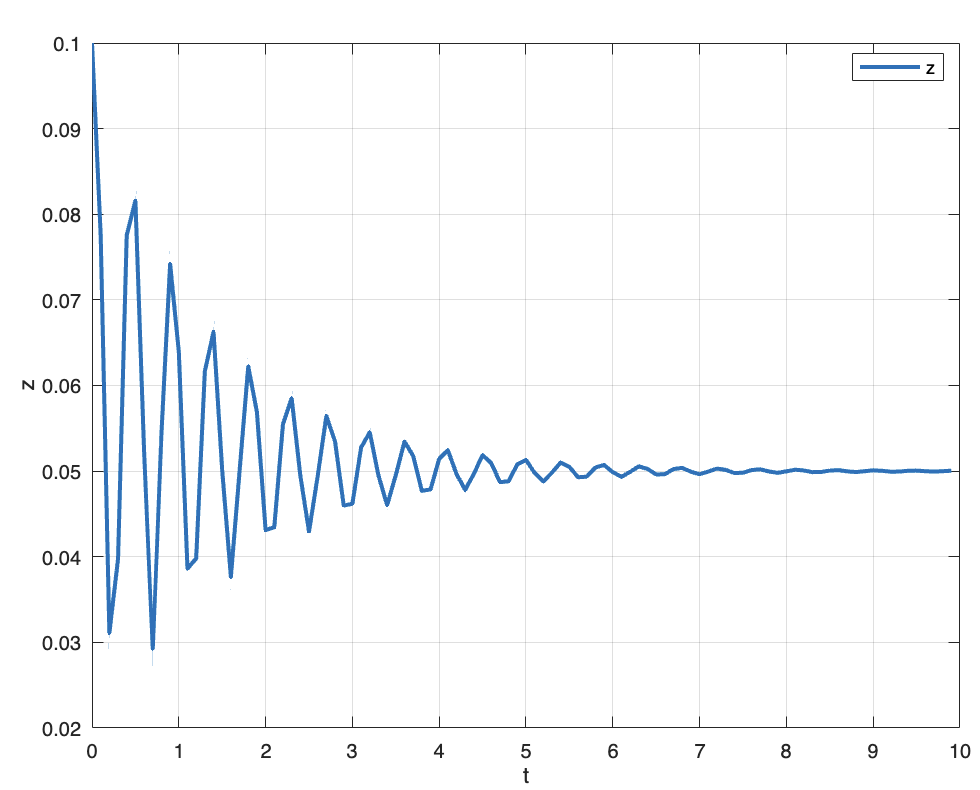
\includegraphics[width = 0.5\textwidth]{Images/simulazione-d-0.1.png}
    \caption{Simulazione $\tilde{z}(0)=0.35$}
    \label{fig:simulazione_d_0.1}
\end{figure}

\spacer
A questo punto simuliamo il sistema al variare di $\tilde{z}(0)$ e verifichiamo che dopo 10 secondi esso si assesti all'altezza di equilibrio.

\begin{figure}[H]
    \centering
    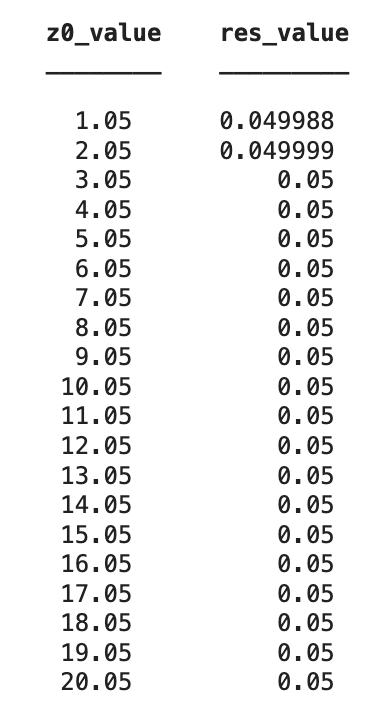
\includegraphics[width = 0.2\textwidth]{Images/risultati-simulazioni.png}
    \caption{Simulazione $\tilde{z}(0) variabile$}
    \label{fig:simulazione_z_variabile}
\end{figure}

\section{Esercizio 2}
Vogliamo disegnare il luogo delle radici della funzione di trasferimento in catena aperta del sistema, per fare questo usiamo mathlab e otteniamo:

\begin{figure}[H]
    \centering
    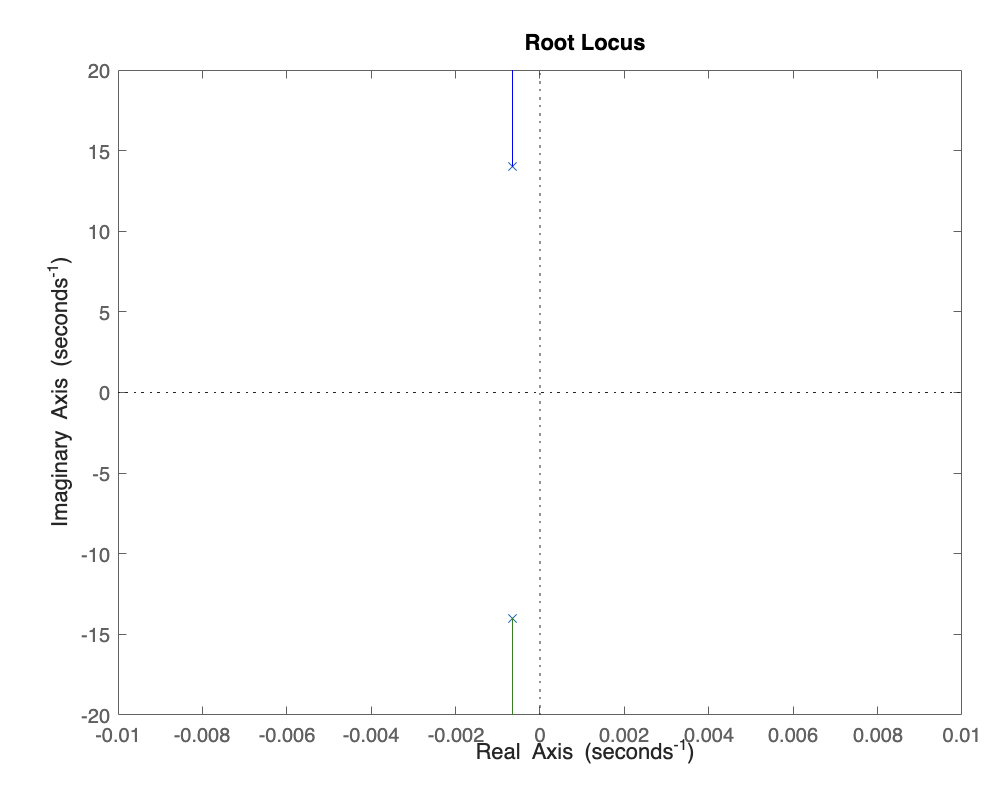
\includegraphics[width = 0.5\textwidth]{Images/luogo-radici-proporzionale.png}
    \caption{Luogo Radice in catena aperta}
    \label{fig:luogo_radice_catena_aperta}
\end{figure}

Per ottenere un controllore con un tempo di salita $T_s \le 1$ vogliamo $T_s = \frac{2}{w_n} \Rightarrow w_n = |p| = 2$

Ma le radici più vicine all'origine hanno $|p| = 14.0071$

Non è quindi possibile costruire un controllore proporzionale con i requisiti richiesti.

\end{document}
